\documentclass[11pt]{article}
\usepackage[margin=1in]{geometry}
\usepackage{booktabs}
\usepackage{array}
\usepackage{multirow}
\usepackage[table]{xcolor}
\definecolor{morblue}{RGB}{218,232,252}
\usepackage{caption}
\usepackage{amsmath}
\usepackage{helvet}
\usepackage{tikz}
\usetikzlibrary{arrows.meta, positioning, shapes.geometric}
\renewcommand{\familydefault}{\sfdefault}

\newcolumntype{R}{>{\raggedleft\arraybackslash}p{1.7cm}}
\captionsetup{font=small, labelfont=bf}

\newcommand{\best}[1]{\textbf{#1}}

\title{\vspace{-2.5em}Recursive Genomic Q-Former:\\ Parameter-Reduction vs.\ Performance Trade-off}
\author{}
\date{}

\begin{document}
\maketitle
\vspace{-3em}

\begin{center}
\setlength{\fboxsep}{10pt}
\fcolorbox{black!40}{black!4}{%
\begin{minipage}{0.94\textwidth}
\textbf{\large Task details}\\[0.4em]
\begin{tabular}{@{}p{3.1cm}p{\dimexpr\textwidth-3.6cm}@{}}
\textbf{Task} & \texttt{cancer\_type} --- 4-way tumor-of-origin classification from bulk
gene-expression profiles (TCGA RNA-seq). \\[0.3em]
\textbf{Dataset} & Unified TCGA cohort: 2{,}738 samples $\times$ 20{,}530 genes; top
4{,}000 highly-variable genes used as input tokens. \\[0.3em]
\textbf{Classes} & Breast (BRCA, 867), Head--neck (HNSC, 423), Lung (LUNG, 943),
Prostate (PRAD, 505). \\[0.3em]
\textbf{Split} & 70/15/15 train/val/test, \textbf{523 test samples}, seed 42. \\[0.3em]
\textbf{Model} & Recursive Genomic Q-Former: $d_{\text{model}}=128$, 256 marker query
slots, recursion depth 4. \\[0.3em]
\textbf{Metric} & Test accuracy and macro-averaged F1. \\
\end{tabular}
\end{minipage}}
\end{center}
\vspace{0.4em}

%---------------------------------------------------------------
\begin{center}
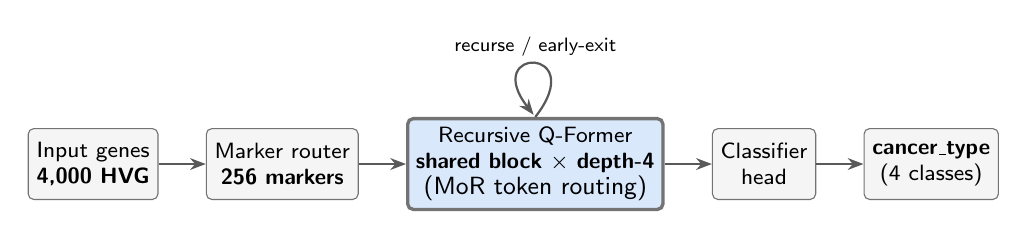
\begin{tikzpicture}[
  node distance=6mm,
  font=\footnotesize,
  box/.style={rectangle, rounded corners=2pt, draw=black!55, fill=black!4,
              minimum height=9mm, align=center, inner sep=3pt},
  mor/.style={rectangle, rounded corners=2pt, draw=black!55, fill=morblue,
              very thick, minimum height=9mm, align=center, inner sep=3pt},
  arr/.style={-{Stealth[length=2mm]}, thick, draw=black!65}
]
\node[box] (in) {Input genes\\\textbf{4{,}000 HVG}};
\node[box, right=of in] (mark) {Marker router\\\textbf{256 markers}};
\node[mor, right=of mark] (rec) {Recursive Q-Former\\\textbf{shared block $\times$ depth-4}\\\small(MoR token routing)};
\node[box, right=of rec] (head) {Classifier\\head};
\node[box, right=of head] (out) {\textbf{cancer\_type}\\(4 classes)};

\draw[arr] (in) -- (mark);
\draw[arr] (mark) -- (rec);
\draw[arr] (rec) -- (head);
\draw[arr] (head) -- (out);

% recursion self-loop on the shared block
\draw[arr, shorten >=1pt] (rec.north) .. controls +(0.7,0.9) and +(-0.7,0.9) .. (rec.north)
  node[midway, above, yshift=-1pt] {\scriptsize recurse / early-exit};
\end{tikzpicture}

\textit{\footnotesize Figure 1: Pipeline. The shared transformer block (blue) is reused
across recursion steps; MoR routes tokens to a per-token depth instead of a fixed pass.}
\end{center}
\vspace{0.6em}

\noindent
All results are on the \textbf{cancer\_type} classification head (4 classes: BRCA, HNSC,
LUNG, PRAD; 523 test samples), with a fixed recursion depth of 4, $d_{\text{model}}=128$,
256 marker query slots, and seed 42. The ``regular'' recursive model shares one
transformer block across all recursion steps; the comparison models either un-tie those
weights (\emph{Independent}) or add token-adaptive routing (\emph{MoR}).

%---------------------------------------------------------------
\begin{table}[h]
\centering
\caption{\textbf{Parameters and performance for all three model types.} One view of the full
trade-off: parameter budget (recurrent-block params, total params, and the independent$/$shared
ratio) alongside all three performance metrics (accuracy, macro-F1, weighted-F1). Sharing the
transformer block cuts recurrent params by $\sim$4$\times$ for a 0.57-point accuracy cost;
Mixture-of-Recursions (MoR) keeps that small budget yet recovers the gap to 0.19 points and is
best on macro-F1.}
\label{tab:main}
\setlength{\tabcolsep}{4.5pt}
\begin{tabular}{l c c r r c r r r}
\toprule
& & & \multicolumn{3}{c}{\textbf{Parameters}} & \multicolumn{3}{c}{\textbf{Performance}} \\
\cmidrule(lr){4-6}\cmidrule(lr){7-9}
\textbf{Model} & \textbf{Weights} & \textbf{Routing} &
\textbf{Recurrent} & \textbf{Total} & \textbf{Ratio} &
\textbf{Acc.} & \textbf{Macro-F1} & \textbf{Wtd-F1} \\
\midrule
Independent stack       & untied & none  & 530{,}432 & 1{,}109{,}897 & 3.99$\times$ & \best{0.9904} & 0.9891 & \best{0.9904} \\
\textbf{Recursive (shared)} & shared & none & 132{,}992 & 712{,}457 & 1.00$\times$ & 0.9847 & 0.9871 & 0.9847 \\
\rowcolor{morblue} \textbf{MoR (token-adaptive)} & \textbf{shared} & \textbf{token} & \textbf{132{,}992} & \textbf{712{,}457} & \textbf{1.00$\times$} & \best{0.9885} & \best{0.9892} & \best{0.9885} \\
\bottomrule
\end{tabular}
\end{table}

\noindent
\textbf{Read-out.} The shared recursive model uses \textbf{74.9\% fewer} transformer
parameters than the independent stack (132{,}992 vs.\ 530{,}432) for a \textbf{0.57-point}
accuracy cost. Adding MoR token routing closes that gap to \textbf{0.19 points} at the same
small parameter budget, and is the only configuration that also reduces FLOPs.

\vspace{1em}
%---------------------------------------------------------------
\begin{table}[h]
\centering
\caption{\textbf{Parameter scaling vs.\ recursion depth.} Shared-weight recursion keeps the
transformer parameter count essentially flat as depth grows, whereas an independent stack
grows linearly. The reduction factor reaches nearly 8$\times$ at depth 8.}
\label{tab:scaling}
\begin{tabular}{c r r c}
\toprule
\textbf{Recursion depth} & \textbf{Shared params} & \textbf{Independent params} &
\textbf{Reduction factor} \\
\midrule
1 & 132{,}608 & 132{,}608   & 1.00$\times$ \\
2 & 132{,}736 & 265{,}216   & 2.00$\times$ \\
4 & 132{,}992 & 530{,}432   & 3.99$\times$ \\
6 & 133{,}248 & 795{,}648   & 5.97$\times$ \\
8 & 133{,}504 & 1{,}060{,}864 & 7.95$\times$ \\
\bottomrule
\end{tabular}
\end{table}

\vspace{1em}
%---------------------------------------------------------------
\begin{table}[h]
\centering
\caption{\textbf{Compute trade-off (depth-4 variants).} Early-exit / adaptive recursion lowers
the \emph{effective} mean depth and FLOPs per sample relative to a fixed depth-4 pass, at equal
parameter count. MoR achieves the lowest compute and the best F1.}
\label{tab:compute}
\begin{tabular}{l r r r r}
\toprule
\textbf{Configuration} & \textbf{Transf.\ params} & \textbf{Mean depth} &
\textbf{MFLOPs/sample} & \textbf{Test acc.} \\
\midrule
Fixed depth-4 (no early exit)   & 132{,}480 & 4.00 & 268.4 & 0.9847 \\
Recursive (shared, early-exit)  & 132{,}992 & 2.75 & 161.5 & 0.9847 \\
No recursive refine             & 132{,}992 & 2.75 & 161.5 & 0.9771 \\
\rowcolor{morblue} \textbf{MoR (token-adaptive)} & \textbf{132{,}992} & \textbf{2.69} & \best{159.1} & \best{0.9885} \\
\bottomrule
\end{tabular}
\end{table}

\vspace{0.5em}
\noindent\footnotesize
\textit{Notes.} Param ratio in Table~\ref{tab:main} is independent$/$shared transformer
parameters. ``Transf.\ params'' counts only the recurrent transformer block (the full model
incl.\ embeddings/heads is $\sim$712K for shared variants, $\sim$1.11M for the independent
stack). Compute-saving for the early-exit and MoR variants is $\approx$40\% of the fixed
depth-4 FLOP budget. Token-reduction at the marker stage additionally compresses 4000 input
genes to 256 retained markers (93.6\% token reduction) at 98.5\% accuracy.

\clearpage
%===============================================================
\section*{Dataset tasks and per-task results}
\normalsize
The model is evaluated on the \textbf{unified TCGA benchmark}: 2{,}738 patient samples,
20{,}530 genes (top 4{,}000 highly-variable genes used as input tokens). The same recursive
architecture (shared block, depth 4, 256 markers) is trained per task. Six prediction targets
span tumor identity, clinical staging, and outcome.

\begin{table}[h]
\centering
\caption{\textbf{Cohort-wise accuracy of the three model types, with parameters.}
\texttt{cancer\_type} is modeled \emph{unified} (pooled across all four cohorts, it \emph{is}
the cohort identity); the five clinical / outcome targets are modeled \emph{separately within
each cohort} (breast, lung, thyroid, head\&neck), for all three model types. Recurrent-block
parameters are listed under each model. Best per row in \textbf{bold}.}
\label{tab:tasks}
\setlength{\tabcolsep}{6pt}
\footnotesize
\begin{tabular}{l l c c c}
\toprule
& & \multicolumn{3}{c}{\textbf{Test accuracy by model}} \\
\cmidrule(lr){3-5}
\textbf{Cohort} & \textbf{Task} &
\textbf{Independent} & \textbf{Recursive (shared)} & \textbf{MoR} \\
& & {\footnotesize 530{,}432 par.} & {\footnotesize 132{,}992 par.} & {\footnotesize 132{,}992 par.} \\
\midrule
\rowcolor{morblue} Unified (all) & \texttt{cancer\_type} & \best{0.9904} & 0.9847 & 0.9885 \\
\midrule
\multirow{5}{*}{Breast (867)}
 & \texttt{pathologic\_stage} & \best{0.4195} & 0.3506 & 0.3333 \\
 & \texttt{pathologic\_T}     & \best{0.5632} & 0.5287 & 0.5287 \\
 & \texttt{pathologic\_N}     & 0.3448 & \best{0.4540} & 0.3333 \\
 & \texttt{os\_binary}        & 0.6782 & 0.5345 & \best{0.7299} \\
 & \texttt{tumor\_status}     & \best{0.8218} & 0.7069 & 0.7356 \\
\midrule
\multirow{5}{*}{Lung (943)}
 & \texttt{pathologic\_stage} & 0.4180 & \best{0.4603} & 0.4392 \\
 & \texttt{pathologic\_T}     & 0.4233 & \best{0.4868} & 0.4709 \\
 & \texttt{pathologic\_N}     & 0.4603 & \best{0.5556} & \best{0.5556} \\
 & \texttt{os\_binary}        & 0.7302 & 0.7778 & \best{0.8519} \\
 & \texttt{tumor\_status}     & 0.6032 & 0.5079 & \best{0.6296} \\
\midrule
\multirow{5}{*}{Thyroid (505)}
 & \texttt{pathologic\_stage} & 0.3168 & 0.2376 & \best{0.3564} \\
 & \texttt{pathologic\_T}     & \best{0.3564} & \best{0.3564} & 0.3267 \\
 & \texttt{pathologic\_N}     & \best{0.6040} & 0.5446 & 0.5743 \\
 & \texttt{os\_binary}        & \best{0.9505} & \best{0.9505} & \best{0.9505} \\
 & \texttt{tumor\_status}     & \best{0.7426} & \best{0.7426} & 0.7030 \\
\midrule
\multirow{5}{*}{Head\&neck (423)}
 & \texttt{pathologic\_stage} & 0.3059 & 0.4824 & \best{0.5765} \\
 & \texttt{pathologic\_T}     & 0.2235 & \best{0.3294} & 0.3176 \\
 & \texttt{pathologic\_N}     & 0.4588 & \best{0.4824} & 0.3059 \\
 & \texttt{os\_binary}        & \best{0.9059} & \best{0.9059} & \best{0.9059} \\
 & \texttt{tumor\_status}     & \best{0.5882} & 0.4706 & 0.4588 \\
\bottomrule
\end{tabular}
\end{table}

\vspace{0.3em}
\noindent\footnotesize
\textit{Notes.} Parameters under each header are recurrent transformer-block parameters
(total $\sim$1.11M Independent; $\sim$712K shared and MoR). All numbers are single-seed
(seed 42) test accuracies. \texttt{cancer\_type} is the unified four-cohort model
(\texttt{results/\{independent,main,mor\_token\}.json}); the per-cohort clinical/outcome
results are from \texttt{results\_cohorts\{\_independent,,\_mor\}/}. Cohort sizes (full,
in parentheses) are split 65/15/20 train/val/test per cohort; with as few as 423 samples and
some rare classes, per-cohort accuracies are noisier than the pooled numbers and no single
model type dominates across cohorts.

\end{document}
